\documentclass[border=10pt]{standalone}

\usepackage{tikz}
\usepackage{tikzsymbols}
\usetikzlibrary{calc,patterns,shapes.geometric}

\def\centerarc[#1](#2)(#3:#4:#5){\draw[#1] ($(#2)+({#5*cos(#3)},{#5*sin(#3)})$) arc (#3:#4:#5);}

\begin{document}
	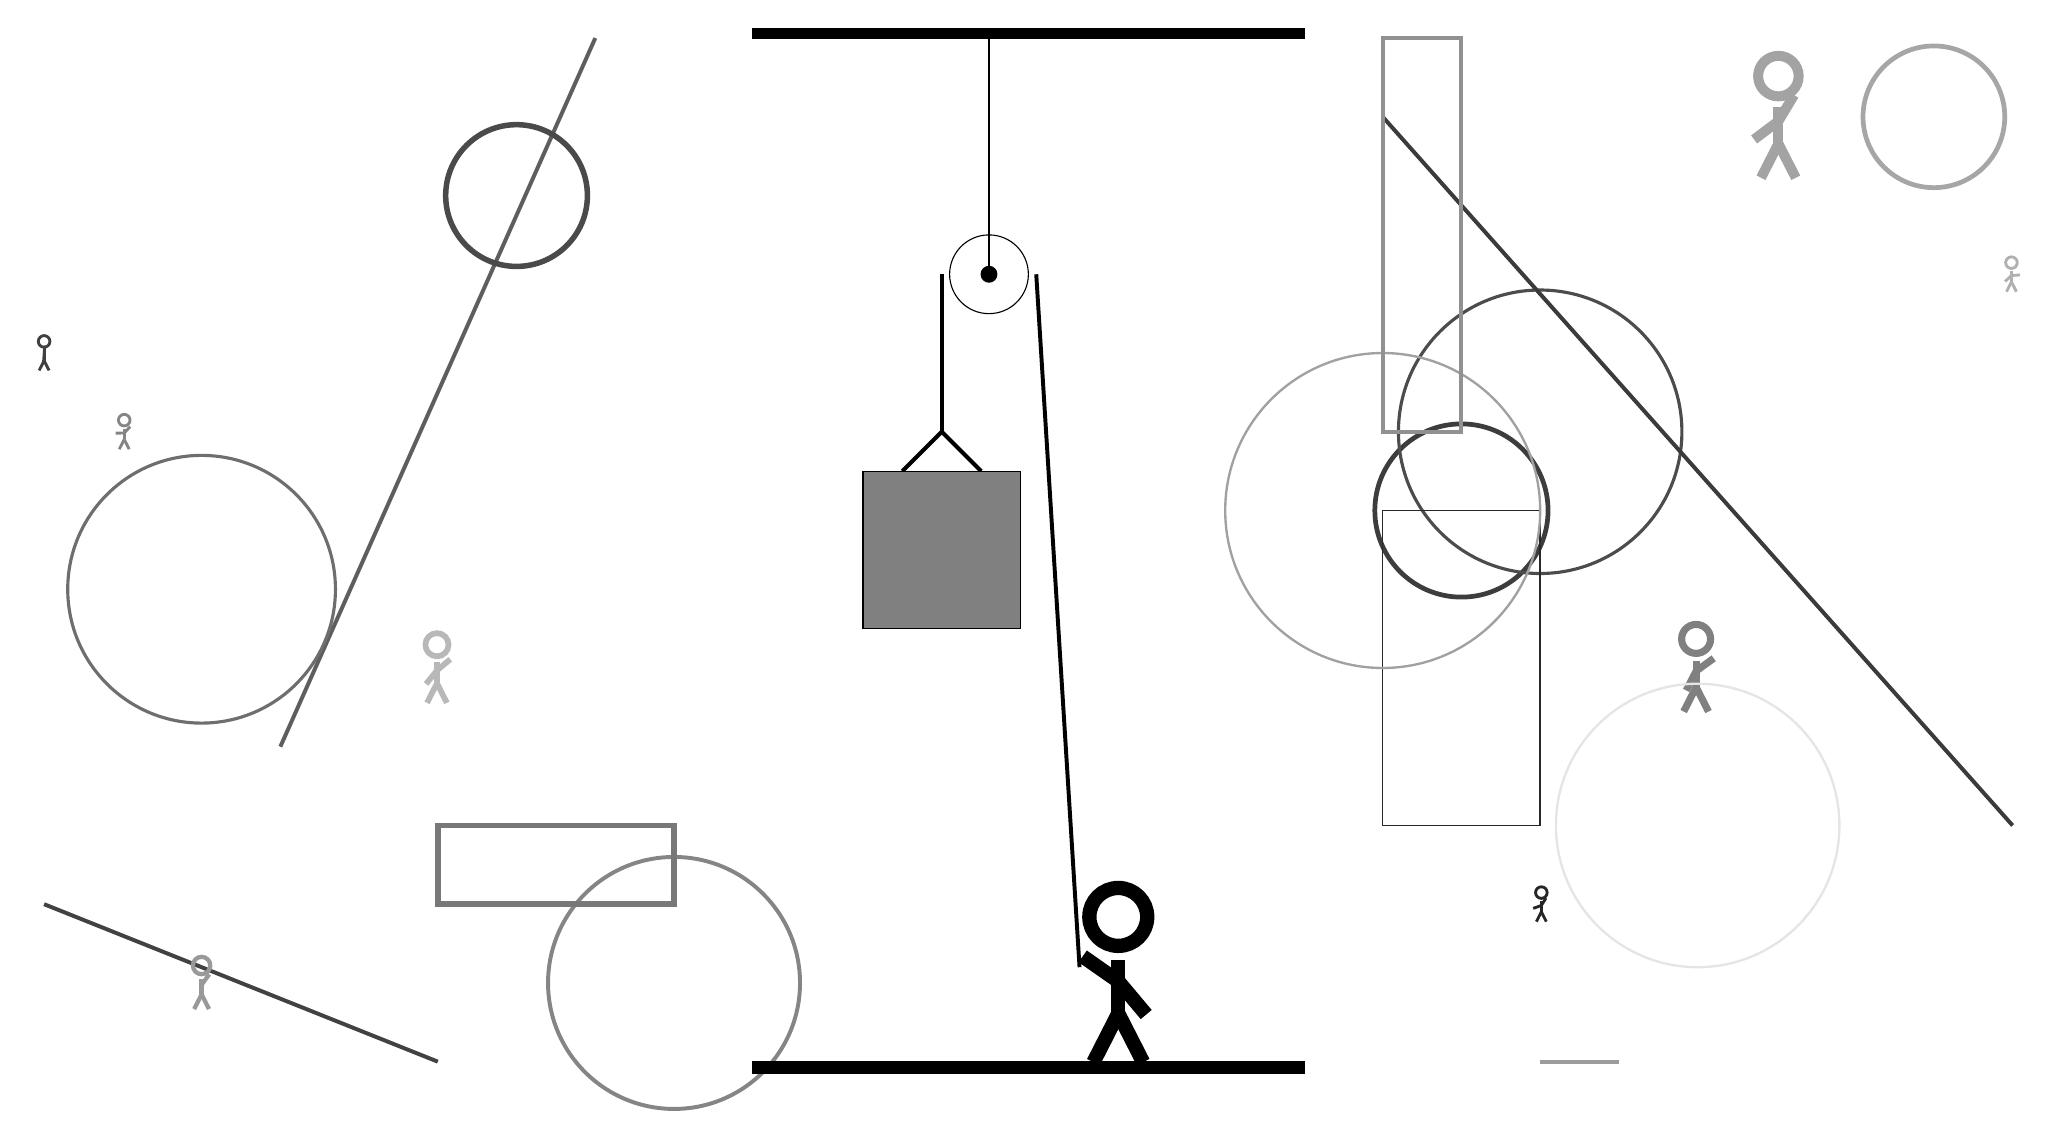
\begin{tikzpicture}
		%%%%% START %%%%%
		
		\draw[fill=black] (-2, 10) rectangle (5, 10.125);
		
		\node[line width=0.7mm, color=black!85] at (8, -1) {\Strichmaxerl[2][20][58]};
		
		\draw [line width=0.6mm, color=black!76](7, 4) circle (1.1);
		\node[line width=0.6mm, color=black!28] at (-6, 2) {\Strichmaxerl[4][51][40]};
		\draw[line width=0.5mm, color=black!63](-4, 10) -- (-8, 1);
		\node[line width=0.6mm, color=black!48] at (-10, 5) {\Strichmaxerl[2][1][47]};
		\node[line width=0.6mm, color=black!50] at (10, 2) {\Strichmaxerl[5][63][36]};
		\node[line width=0.5mm, color=black!31] at (14, 7) {\Strichmaxerl[2][43][4]};
		\draw [line width=0.4mm, color=black!70](8, 5) circle (1.8);
		\draw[line width=0.5mm, color=black!77](6, 9) -- (14, 0);
		\draw[line width=0.2mm, color=black!84] (6, 4) rectangle (8, 0);
		
		\draw[line width=0.5mm, color=black!74](-6, -3) -- (-11, -1);
		\draw [line width=0.2mm, color=black!18](-7, 1) circle (0.0);
		\draw [line width=0.6mm, color=black!35](13, 9) circle (0.9);
		
		\draw [line width=0.3mm, color=black!10](10, 0) circle (1.8);
		\node[line width=0.7mm, color=black!40] at (-9, -2) {\Strichmaxerl[3][88][54]};
		\draw [line width=0.5mm, color=black!48](-3, -2) circle (1.6);
		
		\node[line width=0.7mm, color=black!36] at (11, 9) {\Strichmaxerl[7][37][59]};
		\node[line width=0.2mm, color=black!75] at (-11, 6) {\Strichmaxerl[2][86][86]};
		\draw[line width=0.5mm, color=black!39](9, -3) -- (8, -3);
		
		\draw [line width=0.3mm, color=black!37](6, 4) circle (2.0);
		\draw[line width=0.7mm, color=black!53] (-3, 0) rectangle (-6, -1);
		\draw[line width=0.5mm, color=black!43] (6, 5) rectangle (7, 10);
		\draw [line width=0.4mm, color=black!57](-9, 3) circle (1.7);
		\draw [line width=0.7mm, color=black!71](-5, 8) circle (0.9);
		
		\draw (1, 7) circle (0.5);
		\draw[fill=black] (1, 7) circle (0.1);
		\draw (1, 10) -- (1, 7);
		
		\draw[line width=0.5mm] (-0.1, 4.5) -- (0.4, 5.0) -- (0.9, 4.5);
		\draw[fill=black!50] (-0.6, 4.5) rectangle (1.4, 2.5);
		
		\draw[line width=0.5mm] (0.4, 7) -- (0.4, 5.0);
		\centerarc[line width=0.5mm](1, 7)(0:180:0.6);
		\draw[line width=0.5mm](1.6, 7) -- (2.15, -1.8);
		
		\node at (2.6, -1.9) {\Strichmaxerl[10][-35][-50]};
		
		\draw[fill=black] (-2, -3) rectangle (5, -3.15);
		
		%%%%% END %%%%%
	\end{tikzpicture}
\end{document}